\documentclass[a4paper,12pt]{article}
\usepackage[utf8]{inputenc}
\usepackage[spanish]{babel}
\usepackage{estilosbase}


\title{RobotUI\\ Asistente de diseño de interfaz de control, seguimiento y sharing de robots en tiempo real }
\author{Alumno: Manuel López Urbina\\Director: Arturo Morgado Estévez}
\date{\today}


\begin{document}

% Este archivo es parte de la memoria del proyecto fin de carrera
% de Manuel López Urbina. Protegida bajo la licencia GFDL.
% Para más información, la licencia completa viene incluida en el
% fichero fdl-1.3.tex
% Fuente tomada del PFC 'libgann' de Francisco Javier Vázquez Púa.
% Fuente tomada de la plantilla LaTeX para
% la realización de Proyectos Final de Carrera de Pablo Recio Quijano.
% Copyright (C) 2009 Pablo Recio Quijano

% Copyright (C) 2017 Manuel López Urbina

\pagestyle{empty}
\begin{titlepage}

  \begin{center}

    
\includegraphics[scale=0.2]{inicio/logo_uca.png} \\

    \vspace{2.0cm}

    \LARGE{\textbf{ESCUELA SUPERIOR DE INGENIERÍA}} \\

    \vspace{1.0cm}

    \Large{\textbf{MÁSTER UNIVERSITARIO EN INVESTIGACIÓN EN INGENIERÍA DE SISTEMAS Y DE LA COMPUTACIÓN}} \\

    \vspace{3.0cm}

    \Large{\textbf{ Multi Sensor Robot System (SensorRS), Vehículo robótico multisensorial de exploración controlado por wifi basado en Arduino y Raspberry Pi. }} \\

    \vspace{3.0cm}

    \normalsize{Manuel López Urbina \\
    Director: Arturo Morgado Estévez }\\

    \vspace{1.5cm}
    Cádiz, \today

  \end{center}
\end{titlepage}




\maketitle
\pagestyle{empty}
\abstract{\noindent El siguiente documento se presenta a modo de resumen complementario a la memoria del Proyecto Fin de Carrera de mismo título, entregado el día de la presentación de este proyecto. El proyecto que nos ocupa
trata el desarrollo y puesta de funcionamiento de la aplicación RobotUI. Asistente para el diseño de la interfaz de control, compartición y seguimiento de robots en tiempo real a través de internet acompañado 
 con el desarrollo de un prototipo robótico para la demostración de uso de la aplicación. }
\tableofcontents 

\cleardoublepage
\pagestyle{plain}

\section{Introducción y antecedentes}

La robótica es una rama de la ingeniería, la cual se ocupa del diseño, construcción, operación y uso de robots\footnote{Robot: Máquina automática programable capaz de 
realizar determinadas operaciones de manera autónoma y sustituir a los seres humanos en algunas tareas, en especial las pesadas, repetitivas o peligrosas; puede estar dotada de sensores, 
que le permiten adaptarse a nuevas situaciones.}, así como sistemas informáticos para su control, retroalimentación sensorial y procesamiento de información. Entre las diversas disciplinas aplicadas
a la robótica podemos encontrar: la mecánica, la electrónica, la informática, la inteligencia artificial, la ingeniería de control y la física, entre otras muchas, de lo cual podemos considerar 
la robótica como una ciencia multidisciplinar.\\

En la actualidad, los robots comerciales e industriales son ampliamente utilizados y cada día realizan tareas de forma más exacta o más barata que los humanos. También se les utiliza en trabajos demasiado sucios,
peligrosos o tediosos. Los robots son muy utilizados en plantas de fabricación, montaje y embalaje, en transporte, en exploraciones en la Tierra y en el espacio, cirugía, armamento, investigación en laboratorios y 
en la producción en masa de bienes industriales o de consumo. Otras aplicaciones incluyen la limpieza de residuos tóxicos, minería, búsqueda y rescate de personas y localización de minas terrestres. En definitiva, 
la robótica está presente en prácticamente cualquier ámbito que podamos imaginar.\\

Por otra parte, ninguno de los sistemas robóticos actuales podrían ser funcionales sin un software adecuado para su manejo y control, en ocasiones siendo éste tremendamente complejo y específico para garantizar
una correcta sincronización entre los diferentes elementos hardware y software implicados con la finalidad de garantizar una correcta armonía del conjunto.\\

Por estas razones cada vez son más las escuelas que hacen uso de la robótica para que los estudiantes se interesen en la tecnología, ya que pueden encontrar un entorno divertido donde aprender y que ofrece multitud de ventajas:\\

\begin{enumerate}
\item \textbf{Los niños lo encuentran divertido:} hay varios concursos orientados a distintos grupos de edad que pueden canalizar la competencia de una manera positiva. Por ejemplo, se le puede pedir a los niños que construyan un robot y luego hacer competiciones.\\
\item \textbf{Es una manera eficaz de enseñarles programación a los estudiantes:}
 la programación puede ser muy abstracta. Al tener que controlar un robot físico y ver lo que sale mal, los estudiantes aprenden lo que los robots pueden y no pueden hacer. 
También aprenden la necesidad de dar instrucciones precisas.\\
\item \textbf{ Desarrolla habilidades útiles:}
 capacidad de resolución de problemas, trabajo en equipo, capacidad de análisis, y un largo etcétera.
\end{enumerate}


Actualmente, además, existe una tendencia a la interconexión de aquellos elementos más cotidianos con internet, fenómeno conocido como Internet de las cosas o Internet of things en inglés. Con ello,
se permite el control de multitud de dispositivos, desde gestión de stocks, geolocalización, control remoto, y un largo etcétera de posibilidades. Según la empresa Cisco\footnote{Cisco Systems es 
una empresa global con sede en San José, California, Estados Unidos, principalmente dedicada a la fabricación, venta, mantenimiento y consultoría de equipos de telecomunicaciones.}, en 2020 habrá en
el mundo aproximadamente 50 mil millones de dispositivos con un sistema de conexión al internet de las cosas\footnote{ Estudio referenciado en el libro \textit{Internet of Things - From Research and Innovation to Market Deployment} 
\cite{book:internet_things}.} ¿Por qué no añadir también nuestros proyectos robóticos a la red?.\\

De todo lo anterior se extrae, por tanto, la necesidad de elaborar un sistema que, además de acercar la robótica a los estudiantes, permita compartir sus proyectos con otros usuarios en internet. Todos hemos
visto alguna vez vídeos en las redes sociales donde los usuarios nos muestran sus dispositivos en funcionamiento donde, en ocasiones, nos gustaría poder tomar control sobre ellos o visualizar su manejo en tiempo real.\\

Por tanto el sistema resultante debe cubrir dos necesidades principales, la primera, dotar al usuario de las herramientas necesarias para permitir la configuración de una interfaz de control para 
dispositivos sin necesidad de amplios conocimientos de programación, y la segunda, cubrir la necesidad paralela en la que los usuarios, orgullosos de sus creaciones, dispongan de una manera de 
compartir sus robots con el resto del mundo de una manera más dinámica. Es decir, en la que otros usuarios, a modo de espectadores, puedan visualizar el control de los dispositivos por parte de 
su creador, como si de una sesión de vídeo en streaming se tratara. También se dotará de la posibilidad de permitir el control por otros usuarios externos.\\

Así que dadas las motivaciones existentes y, junto que la programación web y la robótica son temas que causan en mi un especial interés, hicieron que me lanzara a la elaboración de este
proyecto que unifica ambos campos anteriormente citados.\\

Así surgió \emph{RobotUI} y con él un nuevo concepto llamado \textit{RobotSharing}.\\

\begin{figure}[H]
  \begin{center}
    
\includegraphics[scale=0.5]{imagenes/logotipo.png}
  \end{center}
 \caption{Logo RobotUI \protect\footnotemark.}
\end{figure}

\footnotetext{Logotipo RobotUI.}

\emph{RobotUI} (nombre del sistema resultante) será una combinación de un elemento software (aplicación web) y hardware (vehículo de pruebas y demostración) surgido como muestra de la solución obtenida a los citados problemas.\\



\begin{figure}[H]
  \begin{center}
    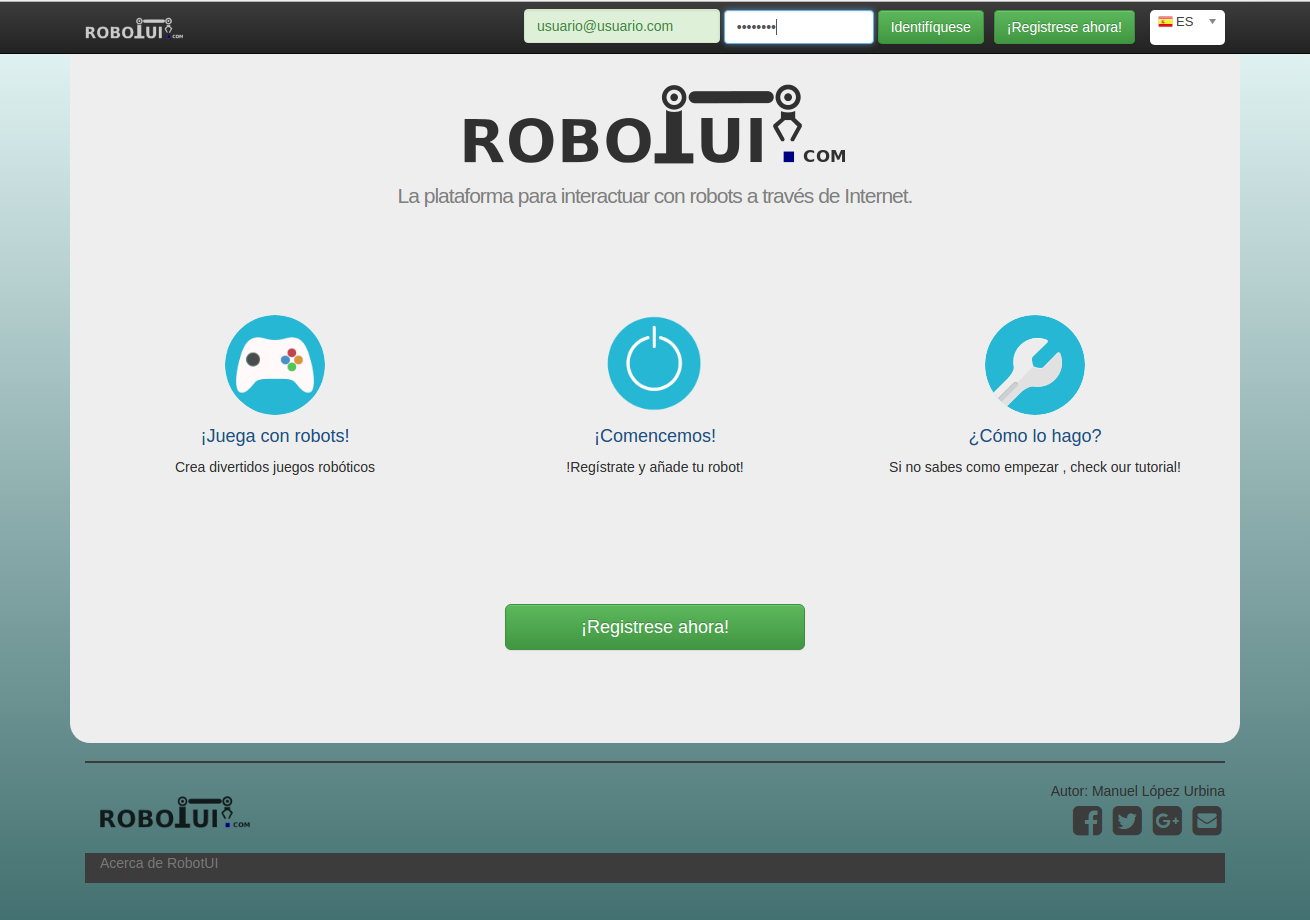
\includegraphics[scale=0.3]{imagenes/pagina-principal.png}
  \end{center}
 \caption{Página principal de RobotUI.}
\end{figure}


El elemento hardware de este proyecto se compone de un vehículo controlado vía WiFi el cual responde a una serie de señales, \emph{comandos}\footnote{ Comando: instrucción u orden que el usuario proporciona a un sistema informático, 
desde la línea de comandos (como una shell) o desde una llamada de programación.}, a los que responde realizando determinadas acciones. Por otra parte también dispone de una cámara para la captura de imágenes\\

La interfaz de control generada en la aplicación web se configurará de tal manera que permita el control del susodicho vehículo a modo demostrativo. Este procedimiento servirá de guía para que cualquier usuario pueda proceder a dar de alta sus dispositivos 
robóticos para su control y difusión con otros usuarios.\\

\begin{figure}[H]
  \begin{center}
    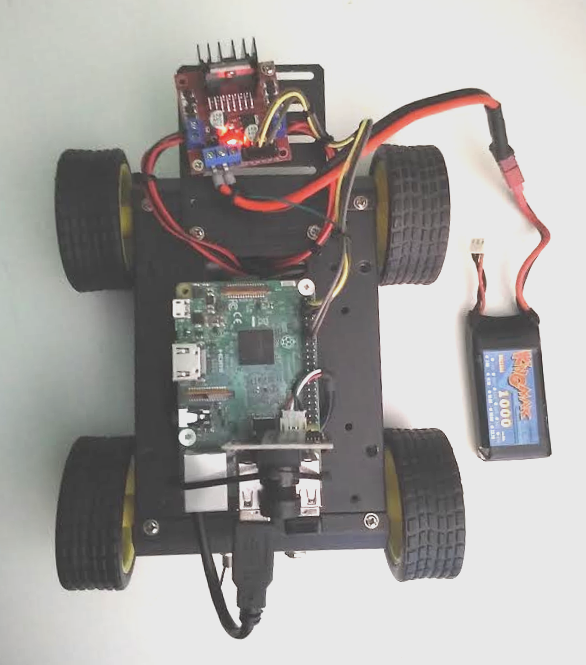
\includegraphics[scale=0.3]{imagenes/robot.jpg}
  \end{center}
  \label{fig:logo}
 \caption{Imagen del vehículo de pruebas desarrollado \protect\footnotemark.}
\end{figure}

\footnotetext{Vehículo desarrollado para probar el funcionamiento de RobotUI. Su desarrollo y características quedan descritas en el capítulo \emph{Robot de pruebas}.}


\section{Objetivos}
\label{sec:objetivos}

Como hemos visto, se requiere de multitud de conocimientos a la hora de afrontar un proyecto robótico con ciertas garantías. Este proyecto trata, al menos, de reducir, o facilitar, el área relacionada con
la informática, más concretamente con la programación donde multitud de personas ven un impedimento a la hora de comenzar a desarrollar sus ideas.\\

Por otro lado, existe la imperiosa necesidad de que los usuarios quieran mostrar sus creaciones al resto del mundo, compartir experiencias, problemas, opiniones, etc, de una forma directa y no
mediante la grabación de vídeos del funcionamiento de los proyectos robóticos en cuestión en la que solo se visualiza su funcionamiento sin la posibilidad de interactuar, ya que no disponen de una herramienta adecuada para ello.\\

De lo anterior deducimos que existe la necesidad de que otros usuarios puedan participar de manera más activa, ya sea visualizando el control del robot por parte de su creador o permitir que otros usuarios
tomen el control de esos proyectos en tiempo real.\\

El sistema a desarrollar dispondrá de dos modos de funcionamiento, el primero de ellos proporciona las herramientas para la configuración de una interfaz a gusto del usuario, en la cual, 
una vez configurada, el usuario podrá controlar a su antojo el dispositivo. En el segundo modo de funcionamiento, la aplicación permitirá que otros usuarios puedan visitar la interfaz anteriormente 
configurada y actuar como espectadores en el control del robot por el usuario propietario del mismo. En definitiva, se proporcionará un sistema de control y difusión en uno solo.\\


En resumen, este proyecto busca facilitar la árdua labor de programación de los proyectos robóticos junto con la posibilidad de compartir las creaciones realizadas con otros usuarios.\\


\section{Acerca de este documento}

El documento se ha sido elaborado en un lenguaje claro y sencillo para permitir que un estudiante universitario de Ingeniería Informática pueda comprender los contenidos sin apenas dificultad añadida.\\

Este documento se organiza en los siguientes capítulos:\\

\begin{itemize}

\item En el capítulo primero, Introducción, se comentan las razones que han motivado la creación de este proyecto, así como el propósito del mismo.

\item En el capítulo segundo, Conceptos básicos, se incluyen definiciones de aquellos conceptos considerados de interés para la correcta comprensión del contenido de la presente memoria.

\item En el capítulo tercero, Estado del arte y herramientas utilizadas, se realiza una descripción de las diferentes elementos hardware y software empleados durante el desarrollo del proyecto y necesarios para la utilización del mismo. Así como una breve descripción del conocimiento acumulado y tecnologías existentes hasta la fecha.

\item En el capítulo cuarto, Desarrollo software, se realiza un análisis sobre la metodología empleada para el desarrollo software, describiendo los modelos de ciclo de vida utilizados, la descripción de los requisitos funcionales y no funcionales junto con los diagramas de casos de uso, de clases y de secuencia.

\item En el capítulo quinto, Desarrollo front-end, se recogen aquellos aspectos técnicos de interés referentes a la elaboración de toda la parte visual de la aplicación.

\item En el capítulo sexto, Comunicaciones, se hace una descripción de las diferentes herramientas proporcionadas por el SDK del framework Sails.js para la gestión de eventos en tiempo real y la descripción de su funcionamiento mediante la explicación de casos prácticos desarrollados en el presente proyecto.

\item En el capítulo séptimo, Robot de pruebas, se recogen aquellos aspectos referentes al montaje, configuración y programación de un robot de pruebas para la demostración y uso de la aplicación desarrollada en el presente proyecto. 

\item En el capítulo octavo, Organización temporal, se recoge todo lo que concierne a la distribución y duración de cada una de las tareas llevadas a cabo durante el desarrollo del proyecto que el presente documento describe.

\item En el capítulo noveno, Guía de usuario, se describen los diferentes aspectos necesarios para la correcta utilización del conjunto software y hardware de los que se compone el presente proyecto.

\item En el capítulo décimo, Comentarios finales, se hace mención de las conclusiones obtenidas tras la realización del proyecto además de las posibles mejoras aplicables y presupuesto.

\item En el capítulo Anexos, aparecen los manuales de instalación del software que ha sido necesario para la realización del proyecto.

\end{itemize}




\section{Herramientas utilizadas}

El presente capítulo recoge información acerca de las diferentes herramientas, tanto hardware como software, utilizadas durante el desarrollo del proyecto y para su posterior utilización. 

\subsection {Herramientas software}


\subsection{Herramientas hardware}

\begin{description}
\item [Vehículo de pruebas ]


\item [Otros elementos]

Entre el resto de dispositivos hardware se han utilizado:

\begin{itemize}
\item Router
\item Cámara, receptor inalámbrico y capturadora de vídeo
\item Capturadora de vídeo
\item Cámara y receptor inalámbrico
\item Gamepad
\item Ordenador
\end{itemize}

\end{description}

\section{Licencia}

La aplicación RobotUI es software libre: usted puede redistribuirlo y/o modificarlo bajo los términos de la Licencia Pública General de GNU según lo publicado por la Free Software Foundation, ya sea la versión 3 
de la Licencia, o (a su elección) cualquier versión posterior.\\

Este programa se distribuye con la esperanza de que sea útil, pero SIN NINGUNA GARANTÍA, incluso sin la garantía implícita de COMERCIALIZACIÓN o IDONEIDAD PARA UN PROPÓSITO PARTICULAR. Ver el GNU
General Public License para más detalles.\\

Debería haber recibido una copia de la Licencia Pública General de GNU junto con este documento. Si no es así, consulte \href{http://www.gnu.org/licenses/}{GNU Licenses}.\\


\section{Conceptos básicos}



\section{Organización temporal}

La planificación general del proyecto siguiendo un modelo SCRUM, empleando para ello el panel de tareas Trello; un gestor de proyectos que permite aplicar una metodología de desarrollo ágil.\\

Cabe destacar que para el desarrollo de RobotUI ha sido necesario emplear varias herramientas, utilidades y bibliotecas. Algunas de ellas ya habían sido utilizadas en ciertas ocasiones, bien sea en el ámbito estudiantil o profesional. 
Sin embargo, otras han requerido un periodo de formación previo, en el que se han adquirido los conocimientos necesarios para poder desarrollar el presente proyecto.\\

La mayor parte del proceso de investigación fue dedicado al estudio de las diferentes tecnologías existentes para la programación web en tiempo real. Todo ello ha implicado un esfuerzo bastante considerable en el uso, 
aprendizaje e investigación de las diferentes tecnologías existentes y comprobar su potencial.\\

Una vez determinadas las diferentes herramientas a utilizar se comenzó con la implementación de la aplicación, siendo seleccionada como herramienta principal el framework Sails.js. Un framework MVC en 
tiempo real para Node.js, el cual está muy enfocado al propósito de este proyecto.\\

Finalmente, tras la necesidad de probar la aplicación en un entorno real, se optó por elaborar un robot de pruebas, un pequeño vehículo elaborado con una Raspberry Pi con la finalidad de probar, testear y hacer 
demostraciones de la aplicación.

La figura \ref{gantt:tareas01} y \ref{gantt:tareas02} muestran una visión de las diferentes tareas desarrolladas para la elaboración del proyecto junto con la descomposición de cada una de ellas:\\

\begin{figure}
  \begin{center}
    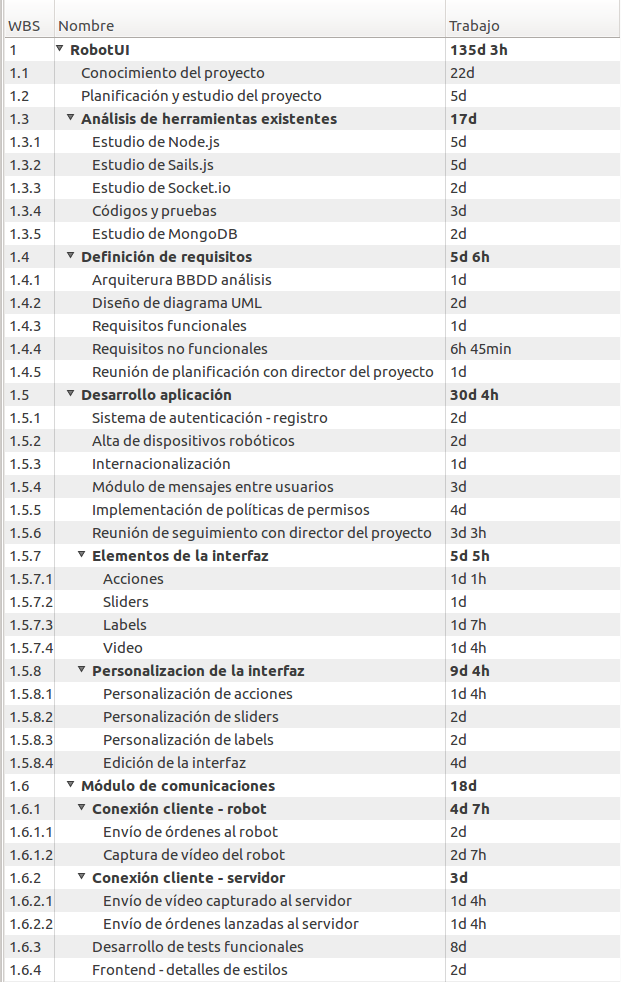
\includegraphics[scale=0.6]{imagenes/descomposicion_tareas01.png}
  \end{center}
  \caption{Descomposición de las tareas implicadas en el desarrollo del proyecto (Primera Parte).}
  \label{gantt:tareas01}
\end{figure}


\begin{figure}
  \begin{center}
    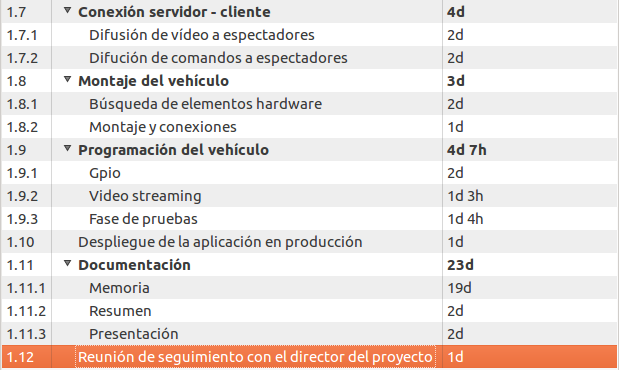
\includegraphics[scale=0.6]{imagenes/descomposicion_tareas02.png}
  \end{center}
  \caption{Descomposición de las tareas implicadas en el desarrollo del proyecto (Segunda parte).}
  \label{gantt:tareas02}
\end{figure}

Los puntos más importantes del proyecto se han dividido en hitos, así como entregas que se definieron en cada reunión que se realizaba con el director del proyecto. 
También se ha definido una planificación temporal del desarrollo del proyecto mediante un diagrama de Gantt con la duración de las tareas recogidas en el panel de actividades de Trello.\\

Los Hitos en los que se ha dividido el proyecto son los siguientes:

\begin{itemize}
 \item Hito 1: Planificación y análisis.
 \item Hito 2: Definición de requisitos.
 \item Hito 3: Comienzo de desarrollo de la aplicación.
 \item Hito 4: Desarrollo de la aplicación, módulo componentes.
 \item Hito 5: Desarrollo de la aplicación, módulo interfaz.
 \item Hito 6: Desarrollo del módulo de comunicaciones.
 \item Hito 7: Construcción del vehículo de pruebas.
 \item Hito 8: Programación del vehículo de pruebas
 \item Hito 9: Documentación.
\end{itemize}


\section{Desarrollo software}

\subsection{Metodología de desarrollo}

Este proyecto ha sido elaborado empleando una metodología de desarrollo basada en el modelo de desarrollo incremental para la parte software referente a todos los subsistemas web y una metodología de 
desarrollo en cascada para el desarrollo de la parte software referente al robot de pruebas.\\

El modelo de desarrollo incremental proporciona una serie de características que lo hacen idóneo para este proyecto. Dicho modelo se basa en la filosofía de construir 
e ir incrementando las funcionalidades del sistema mediante el desarrollo de los diferentes módulos. Esto permite ir aumentando gradualmente las capacidades del software. \\

Dicha metodología de desarrollo resulta especialmente útil en las siguientes situaciones:\\

\begin{itemize}
 \item Facilita el desarrollo permitiendo a cada miembro del equipo desarrollar un módulo particular. En el caso del presente proyecto me ha permitido desarrollar un módulo tras otro de una manera secuencial.
 \item Es similar al ciclo de vida en cascada aplicándose un ciclo en cada nueva funcionalidad del programa.
 \item A final de cada ciclo se entrega el software al cliente. En el caso que compete a este proyecto se mantenía una reunión con el director del proyecto para su aprobación.
\end{itemize}

Centrándonos nuevamente en el desarrollo del proyecto, los motivos que llevaron a cabo la elección de un modelo de desarrollo incremental viene dada por la necesidad de simplificar e ir
desarrollando de una forma gradual y modularizada debido a la extensión del proyecto. Más si cabe que el equipo de desarrollo solo consta de una persona.\\

Por otro lado, para el desarrollo del vehículo de pruebas y por su simplicidad, se ha optado por un desarrollo en cascada. El modelo de desarrollo en cascada resulta adecuado en situaciones
en las que:\\

\begin{itemize}
 \item Se dispone de unos requisitos claros y precisos.
 \item El sistema a desarrollar es de pequeña envergadura.
 \item Las tecnologías utilizadas son conocidas por los desarrolladores.
\end{itemize}

Siendo precisamente éstas las características del del proyecto del vehículo a desarrollar puesto que se trata de un desarrollo de pequeño tamaño y las herramientas empleadas ya me resultaban conocidas
tras la realización de otros trabajos previos.\\

Por tanto el proyecto queda distribuido en los siguientes subsistemas:\\

\begin{figure}[H]
  \begin{center}
    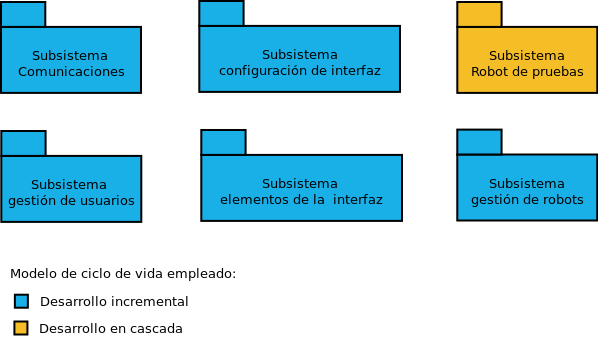
\includegraphics[scale=.6]{imagenes/subsistemas.png}
  \end{center}
  \caption{Subsistemas existentes en el proyecto junto con el modelo de ciclo de vida
utilizado para su desarrollo.}
  \label{website:pagina-principal}
\end{figure}



\section{ Comunicaciones }

En el capítulo de comunicaciones se realiza una introducción sobre el funcionamiento y los fundamentos teóricos sobre cómo se gestionan las diferentes conexiones y eventos de cualquier aplicación
Sails para, posteriormente, centrarse específicamente en la descripción de un caso práctico desarrollado en proyecto con la finalidad de comprender mejor su funcionamiento y poder afianzar
conocimientos.

\section{Introduccion}

Se destacan aquellos aspectos teóricos sobre cómo Sails, framework Node JS utilizado en el desarrollo, trabaja con Websocket y Socket.io y que extraemos a modo resumen.\\

Un servidor HTTP no puede enviar datos a menos que un cliente los haya solicitado mediante una petición. Los Websockets, en cambio, presentan la particularidad de que
permiten que un servidor envíe datos a un cliente sin la necesidad de que éstos sean solicitados, al menos de una manera inmediata. Estas solicitudes, realizadas con anterioridad, se formalizan mediante suscripciones, concepto que 
iremos constantemente haciendo referencia a lo largo del presente capítulo y que debemos recordar.\\

\begin{figure}%
    \centering
    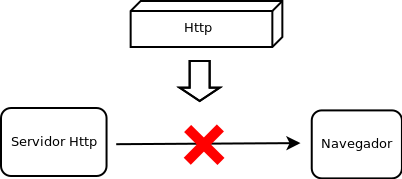
\includegraphics[width=7cm]{imagenes/http-weboscket.png}
    \qquad
    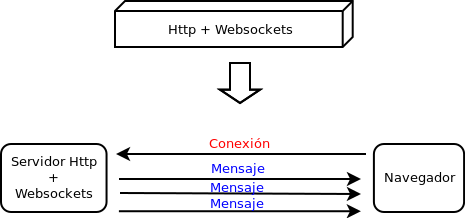
\includegraphics[width=7cm]{imagenes/http+weboscket.png}
    \caption{Peticiones entre un navegador y un servidor HTTP con y sin el empleo de websockets.}%
    \label{fig:http-request}%
\end{figure}

Anteriormente comentamos que el servidor HTTP no puede enviar datos a menos que el cliente lo haya solicitado y los Websockets permiten que un servidor envíe datos no solicitados una vez que se hace 
una conexión inicial (suscripción) desde el lado del cliente. Una aplicación Sails típica queda dividida en dos partes. La primera, en el lado del servidor, consta de un servidor HTTP junto con un nodo
central que actúa como un servidor de sockets.\\ 

En segundo lugar, en el lado del cliente, se dispone de los diferentes códigos HTML y funciones JavaScript para realizar las conexiones con el servidor. Estas conexiones cliente-servidor permiten que 
cualquier otro cliente conectado pueda enviar mensajes al servidor para que a su vez éstos sean emitidos a los clientes que se encuentren conectados en la aplicación en ese instante.\\

Además cada socket posee un identificador único que identifica de manera inequívoca el cliente o, en nuestro, caso el navegador que está accediendo a la página.\\

Destacar también el concepto de salas o rooms de Socket.io. Las salas nos permite agrupar los sockets de modo que en lugar de mensajes que son enviados a todos los sockets conectados, se puede enviar mensajes
sólo a los sockets que están asociados con una sala. De esta podremos mandar mensajes específicos para un cliente concreto, todos ellos o un conjunto de los mismos. \\


\begin{figure}[H]
  \begin{center}
    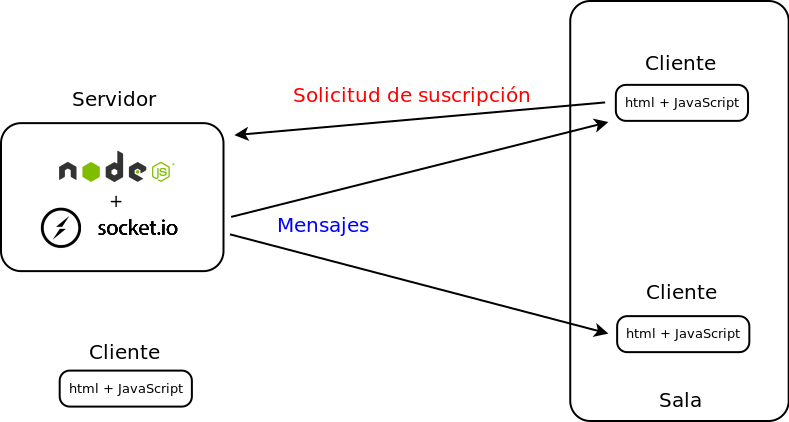
\includegraphics[scale=0.35]{imagenes/salas-websocket.png}
  \end{center}
  \caption{Representación de una sala compuesta por dos clientes.}
  \label{view:userindex}
\end{figure}


De todo los anterior podemos deducir que Sails es un framework especialmente potente, el cual proporciona infinidad de posibilidades a desarrollar. A continuación se cita un fragmento tal y 
como podemos extraer de la página oficial de Sails:\\

\begin{center}
\emph{Sails.js facilita el desarrollo de aplicaciones Node.js empresariales. Ha sido diseñado para imitar el patrón MVC de frameworks como Ruby on Rails, pero con soporte para los requisitos de aplicaciones modernas: data-driven APIs con una arquitectura escalable y service-oriented. Es especialmente bueno para el desarrollo de chats, cuadros de mando en tiempo real o juegos
multijugadores.} 
\end{center}


En este caso menciona diferentes aplicaciones tipo que pueden desarrollarse con Sails, desde un chat, cuadros de mando en tiempo real o juegos multijugadores. RobotUI resulta como una combinación de las 
anteriores puesto que incorpora cuadros de mandos, sistema de mensajería y también es considerado como un juego ya que también está enfocado al entretenimiento.\\


\section{ Interfaz gráfica }


\subsection{Control por parte del usuario}

Lo interesante era proporcionar una serie de mecanismos que permitiera mantener un control del vehículo de una manera cómoda y eficaz para el usuario. Los elementos proporcionados para realizar el control del vehículo son el uso del teclado del ordenador y un gamepad.

\subsection{ Seguimiento por parte del usuario}




\section{Conclusiones}


La elaboración de este proyecto ha resultado muy gratificante a nivel personal. Uno de los motivos principales ha sido la necesidad de trabajar en numerosas áreas de conocimiento entre las que 
encontramos, por un lado la programación web, haciendo uso del framework Sails js, junto con el empleo de una base de datos no relacional. 
Todo ello combinado con la robótica. Algunas de las plataformas mencionadas eran desconocidas al inicio del desarrollo de proyecto y han sido adquiridas tras una amplia labor de investigación.\\

Entre los elementos desarrollados se destaca:

\begin{itemize}
 \item La elaboración de un vehículo de pruebas haciendo uso de una Raspberry Pi 3 Modelo B.
 \item Aprendizaje a la utilización del framework Sails.js.
 \item Aprendizaje al trabajo con eventos en tiempo real mediante el empleo de webSockets, tecnología nunca utilizada por mí hasta la fecha.
 \item Empleo de una base de datos no relacional como Mongo DB.
 \item Transmisión de gran cantidad de datos entre cliente servidor y servidor cliente. Streaming de vídeo y emisión de comandos entre otros datos.\\
\end{itemize}


Pienso que el resultado final del proyecto es ideal para aquellas personas aficionadas a la robótica y programación proporcionando una herramienta sea utilizable por la gran comunidad poseedora 
de cualquier proyecto robótico y que puedan compartirlo con el resto del mundo.\\

Una vez presentado podré continuar añadiendo mejoras y muchas cosas que tengo pensadas y que, posiblemente, se realicen para el proyecto del máster de Ingeniería de Sistemas y Computación que me 
encuentro realizando en la actualidad.\\

\section{Mejoras futuras}

La aplicación puede mejorarse en diversos aspectos. A continuación, se citan algunas de las mejoras que pueden llevarse a cabo:

\begin{itemize}
  \item Permitir la definición de las teclas de control del teclado e incorporación de dispositivos tales como gamepads o joysticks.
  \item Elaborar un generador de código para la exportación a los dispositivos robóticos, reduciendo por tanto las labores de programación. Es decir, proporcionar un generador de código
  en la aplicación de tal manera que a partir de una interfaz elaborada genere el código ejecutable para el robot según su interfaz de control definida\\
  \item Permitir el streaming de audio además del de vídeo.\\
  \item Añadir autenticación por un sistema de certificados por clave pública y privada que garantice que la conectividad entre dispositivo robótico y usuario es la correcta.\\
\end{itemize}


\section{ Guía de Usuario}

El proyecto va acompañado de un manual de usuario, el cual resulta de vital importancia consultar antes y/o durante la utilización de los diferentes elementos tanto hardware, robot de pruebas desarrollado, como software del 
presente proyecto ya que proporciona una guía paso a paso en el manejo correcto de la aplicación.\\

RobotUI ha sido elaborado con un claro propósito; el de  proporcionar a los usuarios un medio donde compartir sus dispositivos robóticos con el resto de usuarios. Esto es posible gracias a una serie de
herramientas desarrolladas para que, sin necesidad de tener grandes conocimientos en programación, puedan configurar un entorno para el manejo de sus proyectos robóticos y tener 
posibilidad de compartir sus dispositivos y experiencias con el resto de usuarios.\\

La particularidad de RobotUI es que el usuario propietario del robot tiene la posibilidad de permitir el manejo de sus dispositivos robóticos al resto de usuarios que él mismo considere de una 
manera controlada o, por otra parte, permitir que otros usuarios visualicen, como si de espectadores se tratase, el control que un determinado usuario realiza de un determinado robot.
Todo ello en tiempo real.\\

Por tanto, tras esta breve introducción en el ámbito de la aplicación, en el manual se describen los diferentes pasos a realizar para configurar los dispositivos correctamente en el sistema
y abrirlo a toda una comunidad de usuarios. Además de tener abierto el acceso a otros muchos dispositivos de otras personas.\\

\subsection{ Objetivos de la guía de usuario }

La guía de usuario tiene como objetivo proporcionar al usuario un soporte de ayuda e iniciación a la utilización de RobotUI.\\

Comprende de las siguientes secciones:\\

\begin{itemize}
 \item Introducción.
 \item Guía de acceso al código fuente de la aplicación.
 \item Guía de uso de la aplicación.
 \item Guía para la puesta en marcha y programación de un robot.
\end{itemize}

\clearpage
\nocite{*}

\bibliography{resumen}{}
\bibliographystyle{plain}
\pagestyle{empty}


\end{document}
